%!TEX TS-program = xelatex
\documentclass[]{friggeri-cv}
\usepackage{afterpage}
\usepackage{hyperref}
\usepackage{color}
\usepackage{xcolor}
\hypersetup{
    pdftitle={},
    pdfauthor={},
    pdfsubject={},
    pdfkeywords={},
    colorlinks=false,       % no lik border color
   allbordercolors=white    % white border color for all
}
\addbibresource{bibliography.bib}
\RequirePackage{xcolor}
\definecolor{pblue}{HTML}{0395DE}

\usepackage{enumitem}

\begin{document}
\header{Victor M.}{Mendiola-Lau}{Computer Scientist, Researcher, Software Developer}
      
% Fake text to add separator      
\fcolorbox{white}{gray}{\parbox{\dimexpr\textwidth-2\fboxsep-2\fboxrule}{%
.....
}}

% In the aside, each new line forces a line break
\begin{aside}
  \section{Address}
    Ayuntamiento 7375, 
    Havana, Cuba
    ~
  \section{Telephone}
    (+53)5 413 2909 (cell)
  	(+53)7 873 0125 (home)
    ~
  \section{Mail}
    \href{mailto:ryuzakyl@gmail.com}{\textbf{ryuzakyl@}gmail.com}
    ~
  \section{Web profiles}
    \href{https://github.com/ryuzakyl}{{\scriptsize github.com/ryuzakyl}}
    \href{https://independent.academia.edu/VictorMendiolaLau}{{\scriptsize academia.edu/VictorMendiolaLau}}
    \href{https://www.linkedin.com/in/VictorMendiolaLau}{{\scriptsize linkedin.com/in/VictorMendiolaLau}}
	\href{https://www.researchgate.net/profile/Victor_Mendiola-Lau}{{\scriptsize researchgate.net/Victor\char`_Mendiola-Lau}}
    ~
  \section{Personal Skills}
    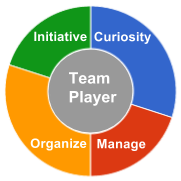
\includegraphics[scale=0.62]{img/personal.png}
    ~
  \section{Languages}
  	\textbf{English}
\includegraphics[scale=0.40]{img/5stars.png}
  	\textbf{Spanish}
\includegraphics[scale=0.40]{img/5stars.png}
    \textbf{French}
\includegraphics[scale=0.40]{img/4stars.png}
	~
  \section{Programming}
    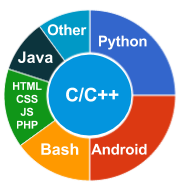
\includegraphics[scale=0.62]{img/programming.png}
    ~
  \section{OS Preference}
    \textbf{GNU/Linux}
\includegraphics[scale=0.40]{img/5stars.png}
    \textbf{Windows}
\includegraphics[scale=0.40]{img/4stars.png}
    \textbf{MacOS}
\includegraphics[scale=0.40]{img/4stars.png}
    ~
\end{aside}

\section{Experience}
\begin{entrylist}
  \entry
    {02/13 - Now}
    {Software Engineer}
    {Fluidmesh Networks SRL, Milano, Italy}
    {Design and development of algorithms, solutions and high speed mobility           schemes for Wireless Mesh Networks. Design and development of embedded software     for Wireless Network devices.\\}
  \entry
    {01/12 - 01/13}
    {Freelance Developer \& Consultant}
    {Icosaedro Solutions}
    {Design and development of Android Applications, Web Solutions, Unix and GNU/Linux software.\\}
    \entry
    {12/09 - 06/09}
    {Project Manager and Webmaster}
    {D.I.D.A.G., Grassano (MT), Italy}
    {Design, development and management of an e-commerce website on Joomla!1.5 CMS platform.\\}
    \entry
    {06/09 - 09/09}
    {Part-time collaboration}
    {Area Sistemi Informatici, Università di Pisa, Italy}
    {Computer technical support. Problem solving related to hardware, software and Operating Systems. Management of the internal network.\\}
    \entry
    {06/09 - 09/09}
    {Internship}
    {Atitlan Engineering SRL, Pisa, Italy}
    {Management and migration of servers. Development of web templates and interfaces. Management of SQL databases.}
\end{entrylist}

\section{Education}
\begin{entrylist}
  \entry
    {2009 - 2012}
    {Master's Degree in Computer Engineering}
    {Università di Pisa, Italy}
    {Curriculum Networking and Multimedia.\\
    Main subjects: Network Applications, Systems Architecture and Security, Mobile Applications, Multemedia Information            Processing.\\
    \emph{Title of the Thesis: "A Handoff Algorithm based on Link Quality Prediction for Mass Transit Wireless Mesh Networks"      .}\\
    \emph{Relators: Prof. Enzo Mingozzi, Ing. Carlo Vallati, Prof. Luciano Lenzini.}\\}
  \entry
    {2005 - 2009}
    {Bachelor's Degree in Computer Engineering}
    {Università di Pisa, Italy}
    {Main subjects: Matematics and Physics, Programming, Operational Research, Telecommunication Systems, Digital and Analogical Electronics.\\
    \emph{Title of the Thesis: "Development, Management and Migrations of web contents and applications".}\\
    \emph{Thesis activity carried out during an internship period at Atitlan Engineering SRL.}\\}
  \entry
    {2000 - 2005}
    {Scientific Disploma.}
    {Liceo Scientifico, Matera, Italy}
    {Scientific Secondary School.\\
    Main subjects: Matematics, Physics, Computer Science.}
\end{entrylist}

%\section{Certifications}
%\begin{entrylist}
%  \entry
%    {02/2013}
%    {Intro to Computer Science}
%    {Udacity. E-learning}
%    {\emph{Building a Python Search Engine}}
%\end{entrylist}
%\newpage

\section{Publications}
\begin{entrylist}
  \entry
    {2017}
    {}
    {}
    {
		% Paper written for journal.\\
	
		Paper accepted on CIARP 2017 Conference.    
    }
\end{entrylist}

\begin{entrylist}    
  \entry
    {2016}
    {}
    {}
    {
		\textbf{Victor Mendiola-Lau}, F.J. Silva-Mata, Y. Martínez-Díaz, I. Talavera Bustamante and M. De Marsico. ``Exploratory Data Analysis Combined with Entropy-based Template Selection for the Identification of Mixed Substances."	 \emph{CAC}, 2016.\\
	
		\textbf{Victor Mendiola-Lau}, Francisco J. Silva Mata, Yoanna Martínez-Díaz, Isneri Talavera Bustamante, Maria De Marsico. ``Hierarchical Clustering Combined with Entropy Based-template Selection and SVM Classification for the Identification of Mixed Substances by Means of UV and GC Analytical Technique." \emph{Informática}, 2016.\\	
	
		\textbf{Victor Mendiola-Lau}, Francisco J. Silva Mata, Yoanna Martínez-Díaz, Isneri Talavera Bustamante and Maria De Marsico. ``Automatic classification of herbal substances enhanced with an entropy criterion." \emph{CIARP}, 2016.  
    }
\end{entrylist}

\begin{entrylist}    
  \entry
    {2015}
    {}
    {}
    {
		Francisco J. Silva-Mata, \textbf{Victor Mendiola-Lau}, Isneri Talavera-Bustamante and Yoanna Martínez-Díaz. ``Automatic processing of TLC images for discovering clusters and performing classification tasks of herbal substances. Case of study". \emph{SSC14}, 2015.\\
	
		Francisco J. Silva Mata, Dania P.- Muñoz, Stefano Berretti, \textbf{Victor Mendiola-Lau}, Isneri Talavera Bustamante, Noslen Hernández, Yoanna Martínez-Díaz, Angel Augier . ``Alineación de señales e imágenes durante la aplicación del análisis de datos funcionales: Ejemplos prácticos en señales e imágenes quimiométricas y biométricas."  \emph{RCF}, 2015.\\
	
		Francisco J. Silva Mata, Dania P.- Muñoz, \textbf{Victor Mendiola-Lau}, Isneri Talavera Bustamante, Angel Augier. ``Criterios y métodos de selección de bases y su impacto en el análisis de datos funcionales: Algunos ejemplos en biometría". \emph{RCF}, 2015.\\
	
		\textbf{Victor Mendiola-Lau}, Isneri Talavera Bustamante and Maria de Marsico. ``Clustering of simple and multi-way spectral data on the dissimilarity representation." \emph{Serie Azul CENATAV}, 2015.\\
	
		Francisco J. Silva Mata,  Isneri Talavera, \textbf{Victor Mendiola-Lau}, Yoanna Martínez Díaz, Anier Revilla Eng. ``Clasificación de Sustancias Vegetales con el uso de un Sistema Automatizado para el proceso de Imágenes de TLC". En: IX Congreso de Ciencias, Tecnología e Innovación Química, Quimicuba 2015, La Habana, Cuba, 13-16 de octubre de 2015.\\
	
		Dania Porro, Isneri Talavera, Robert Duin, Gabriela Barcas, \textbf{Victor Mendiola-Lau}. ``Comparación De Diferentes Formas De Representación De Datos Espectrales Para Clasificación De Sustancias." En: IX Congreso de Ciencias, Tecnología e Innovación Química, Quimicuba 2015, La Habana, Cuba, 13-16 de octubre de 2015.\\
	
		Francisco J. Silva Mata, \textbf{Victor Mendiola-Lau}, Anier Revilla, Isneri Talavera, Angel Augier, Stefano Berretti y Yoanna Martínez. Optimización de los Modelos Funcionales para Objetos Biométricos. \emph{RECPAT}, 2015.   
    }    
\end{entrylist}

\begin{entrylist}   
  \entry
    {2014}
    {}
    {}
    {
		Francisco J. Silva-Mata, Dania P.-Muñoz, \textbf{Victor Mendiola-Lau}, Isneri Talavera-Bustamante, Angel Augier. ``Criteria and methods of selection of bases and their impact in functional data analysis. Some examples in biometrics". \emph{CIOFF}, 2014.\\
	
		Francisco J. Silva-Mata, Dania P.-Muñoz, Stefano Berretti, \textbf{Victor Mendiola-Lau}, Isneri Talavera-Bustamante, Noslen Hernández, Yoanna Martínez-Díaz, Angel Augier. ``Signal and image alignment during the application of functional data analysis. Practical examples of chemometrics and biometrics". \emph{CIOFF}, 2014.\\

		\textbf{Victor Mendiola-Lau}, Francisco J. Silva-Mata, Dania P.-Muñoz, Isneri Talavera-Bustamante. ``APIris: Nueva Plataforma Automatizada para el Reconocimiento de Iris". \emph{RECPAT}, 2014.\\

		Francisco J. Silva-Mata, Dania P.-Muñoz, \textbf{Victor Mendiola-Lau}, Anier Revilla-Eng, Isneri Talavera-Bustamante. ``Criterios y métodos para representar imágenes biométricas usando FDA". \emph{RECPAT}, 2014. 
    }
\end{entrylist}

\begin{entrylist}
  \entry
    {2013}
    {}
    {}
    {
		Dania P.-Muñoz, Francisco J. Silva-Mata, \textbf{Victor Mendiola-Lau}, Noslen Hernández, and Isneri Talavera-Bustamante. ``A new iris recognition approach based on a functional representation". \emph{CIARP}, 2013. 
    }
\end{entrylist}

\begin{entrylist}
  \entry
    {2011}
    {}
    {}
    {
		Javier Guillot-Jiménez, \textbf{Victor Mendiola-Lau}, Benny Jon-Robaina, Daniel A. Mesejo-León, Omar Salas-García and Haydée Guillot-Jiménez. ``SIMPLER: SIMPLER: desde el MERX hasta las Bases de Datos". \emph{COMPUMAT}, 2011.   
    }
\end{entrylist}
\\
\section{Other Info}
\begin{entrylist}
  \entry
    {2001}
    {Valedictorian from my Elementary School}
    {}
    {}
\end{entrylist}

%For the Italian job market:\\
%\emph{Si autorizza il trattamento delle informazioni contenute nel curriculum in conformità alle disposizioni previste dal d.lgs. 196/2003. Si dichiara altresì di essere consapevole che, in caso di dichiarazioni non veritiere, si è passibili di sanzioni penali ai sensi del DPR 445/00 oltre alla revoca dei benefici eventualmente percepiti.}
%\\
%\begin{flushleft}
%\emph{January 14th, 2014}
%\end{flushleft}
%\begin{flushright}
%\emph{Carmine Benedetto}
%\end{flushright}

%%% This piece of code has been commented by Karol Kozioł due to biblatex errors. 
% 
%\printbibsection{article}{article in peer-reviewed journal}
%\begin{refsection}
%  \nocite{*}
%  \printbibliography[sorting=chronological, type=inproceedings, title={international peer-reviewed conferences/proceedings}, notkeyword={france}, heading=subbibliography]
%\end{refsection}
%\begin{refsection}
%  \nocite{*}
%  \printbibliography[sorting=chronological, type=inproceedings, title={local peer-reviewed conferences/proceedings}, keyword={france}, heading=subbibliography]
%\end{refsection}
%\printbibsection{misc}{other publications}
%\printbibsection{report}{research reports}

\end{document}
